\fig{fv:m3:exit}{圆轨迹只是候选延拓，物理轨迹在首次有效出界处切换}{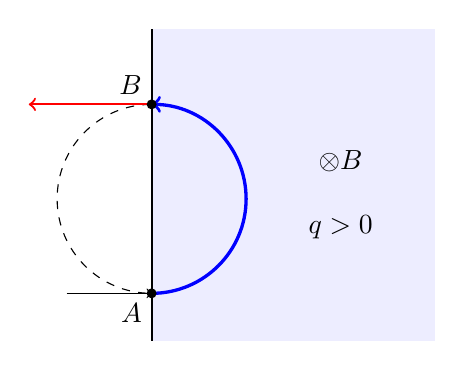
\begin{tikzpicture}[scale=1.2]
\fill[blue!7](1,-.5)rectangle(4,2.8);\draw[thick](1,-.5)--(1,2.8);\draw[dashed](1,1)circle(1);
\draw[->,blue,very thick](1,0)arc(-90:90:1);\draw[->,red,thick](1,2)--(-.3,2);
\draw[->](.1,0)--(1,0);\fill(1,0)circle(1.5pt)node[below left]{$A$};\fill(1,2)circle(1.5pt)node[above left]{$B$};
\node at(3,1.4){$\otimes B$};\node at(3,.7){$q>0$};\end{tikzpicture}}
图\ref{fv:m3:exit}中正电荷由 $A$向右进入磁场，洛伦兹力最初向上，圆心在入射点正上方。只有右半圆处于磁区，第一次回到边界的 $B$才是出界事件；此后沿切线直飞，不能继续沿虚线圆周运动。求有限磁区题时，先由入射位置和力方向定圆心，再按转动方向排列各边界交点；最小正飞行时间对应的有效交点才能连接下一阶段。
